\documentclass{article}
\usepackage{pgfplots}
\pgfplotsset{
    compat=1.18,
    %width=5cm,
    mygraph/.style={
        small,
        xlabel={Tiempo [s]},
        ylabel={Posición [m]},
        xmin=0, xmax=20,
        axis lines=left,
        axis line style={thick},
        xtick distance=5,
        ytick distance=10,
        grid=major,
        grid style={solid,gray},
        width=6cm
    }
    }

\begin{document}
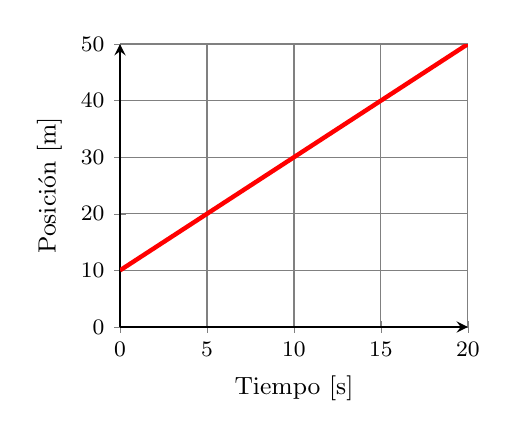
\begin{tikzpicture}
    \begin{axis}[mygraph, ymin=0, ymax=50,]
        \addplot[
            color=red,
            style=ultra thick,
            domain=0:30,
        ] {10 + 2*x};
    \end{axis}
\end{tikzpicture}
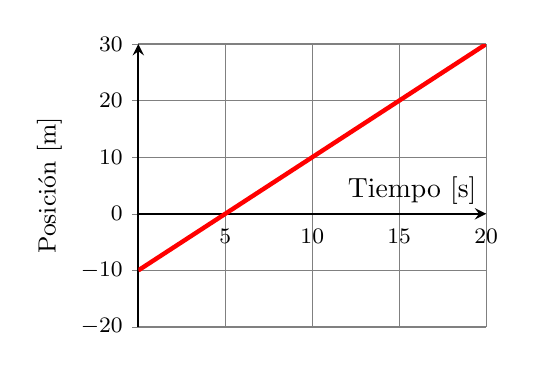
\begin{tikzpicture}
    \begin{axis}[mygraph, ymin=-20, ymax=30, axis x line=middle,]
        \addplot[
            color=red,
            style=ultra thick,
            domain=0:20,
        ] {-10 + 2*x};
    \end{axis}
\end{tikzpicture}
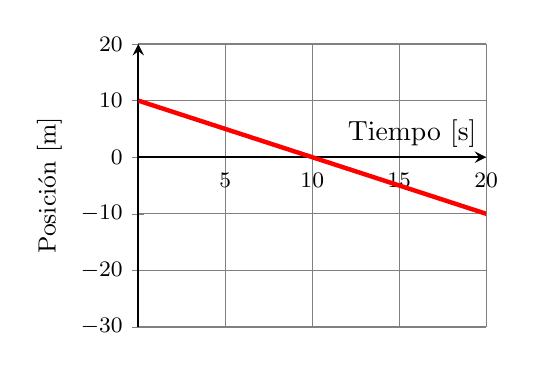
\begin{tikzpicture}
    \begin{axis}[mygraph, ymin=-30, ymax=20, axis x line=middle,]
        \addplot[
            color=red,
            style=ultra thick,
            domain=0:30,
        ] {10 - x};
    \end{axis}
\end{tikzpicture}
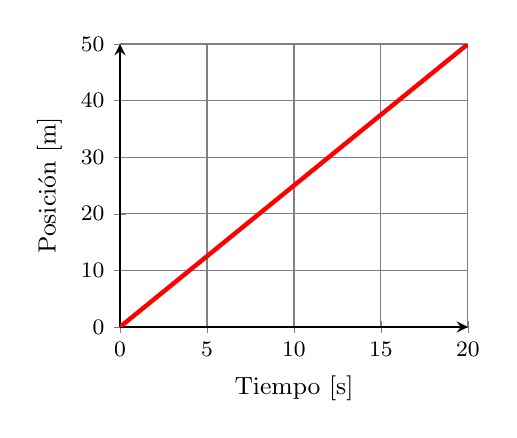
\begin{tikzpicture}
    \begin{axis}[mygraph, ymin=0, ymax=50,]
        \addplot[
            color=red,
            style=ultra thick,
            domain=0:30,
        ] {2.5*x};
    \end{axis}
\end{tikzpicture}
\end{document}